\chapter{Roadmap for further development}
This chapter describes what work remains in this project and a pointer to how this could be done. The different points of improvement mentioned in this chapter provides an overview of what the group would have focused on if given more time.

\section{The $\mu$C Software Store application}
This section focuses on areas of improvement regarding the $\mu$C Software Store. Some of the points mentioned in this section are important to elaborate on for the application to be fully usable to the general user, while others are of less importance.

	\subsection{Database}
	One of the most pressing matters that needs to be elaborated in future work is the implementation of a remote database. The delivered version of the application uses a local database that is automatically filled with data when the application is installed on an Android device. The use of a local database makes it difficult for general users of the application to add their personal apps to the $\mu$C Software Store database. This is because these apps would need to be hard coded into the Android application. With more time available, the group would have implemented a remote database that would contain all the apps that would be offered through $\mu$C Software Store. Content providers and sync adapters provided by Ubibazaar could be used to achieve this.

	\subsubsection{Uploading interface}
	Although outside the scope of the assignment given for the project, future work should encompass implementing an interface for easy uploading of apps to the $\mu$C Software Store. A possible solution for this could be something like the system used by Google Play. Here, registered users easily can submit and upload their own application through a web interface provided by Google Play. Allowing users to upload their own apps would enrich the product greatly, opening for a much wider user group.\\
	\newline
	It is envisioned that the use of a separate web site for uploading of apps would be best for this solution. On this web site the users should be able to view the existing apps in the database as well as submitting their own; much like \textit{http://play.google.com}.

	\paragraph{Security.} Allowing individual developers to upload their own apps to the database would require an administrator or moderator to review the submitted apps. This is important to avoid uploading of malicious apps and duplicates in the system.

	\subsection{Standard for defining $\mu$C Software Store compatible microcontroller-based devices}
	As part of the assignment, the group was supposed to implement filtering of apps that is incompatible with the connected device. As mentioned in section~\ref{removals} this requirement was omitted due to lack of time. Instead of implementing the actual filtering into the application, it was decided that the group should produce a standard for defining $\mu$C Software Store compatible microcontroller-based devices. This standard can be viewed in appendix~\ref{microcontroller_standard}. \\
	\newline
	Future work should encompass implementing this, or a similar standard, into the $\mu$C Software Store. Allowing users to filter apps according to compatibility with the connected device will empower the application and increase its usability.

	\subsection{Performance}
	Given more time, the group would have had a higher focus on the performance of the $\mu$C Software Store. Although the performance is satisfactory, it is possible to enhance it. Future work on this issue should encompass profiling the application to identify non-optimized sections in the code. Optimization of battery usage should also be looked into.

	\subsection{GUI}
	The Android developer design guide teaches the developers of Android applications how to design applications that fits the Android platform. Further work on the $\mu$C Software Store should make sure that the application follows the design guidelines provided by the Android Developer Guide~\cite{android-dev-guide}. This implies correct use of colours, scaling of the application to fit different screen sizes, use of patterns etc.

\section{STK500 and over-the-air installation}
This section focuses on the areas of improvement regarding the implementation of the STK500 protocol, and over the air installation of apps on Arduino. Although the functional requirements set by the customer were met and it is possible to  install apps on an Arduino using the $\mu$C Software Store, there are still some areas of improvement.

	\subsection{Hard reset}
	There was not enough time to fully implement neither the hardware- nor the software implementations of hard reset. The former due to soldering difficulties and lacking documentation, and the latter had to wait for the former (though
    sections in the code where the feature should be enabled was identified).

	   \subsubsection{How to hard reset}
    	Both Bluetooth devices experimented on (RN-42~\cite{rn-42} and HC-05~\cite{hc-05}) provide pins that can be used for detecting when it makes a connection. Passing the output to the reset pin of the microcontroller (coupled with a
        transistor to make it able to coexist with the soft reset) will then cause it to reset, as shown in Figure~\ref{fig:hardReset}. The group has confirmed that this will work.\\

        Triggering a hard reset is then as simple as disconnecting from the Bluetooth device and then reconnecting
        again. Timing is important, however, as the protocol code must communicate with the boot loader before
        the latter attempts to start the installed app.

		\begin{figure}[H]
		\centering
		\label{fig:hardReset}
		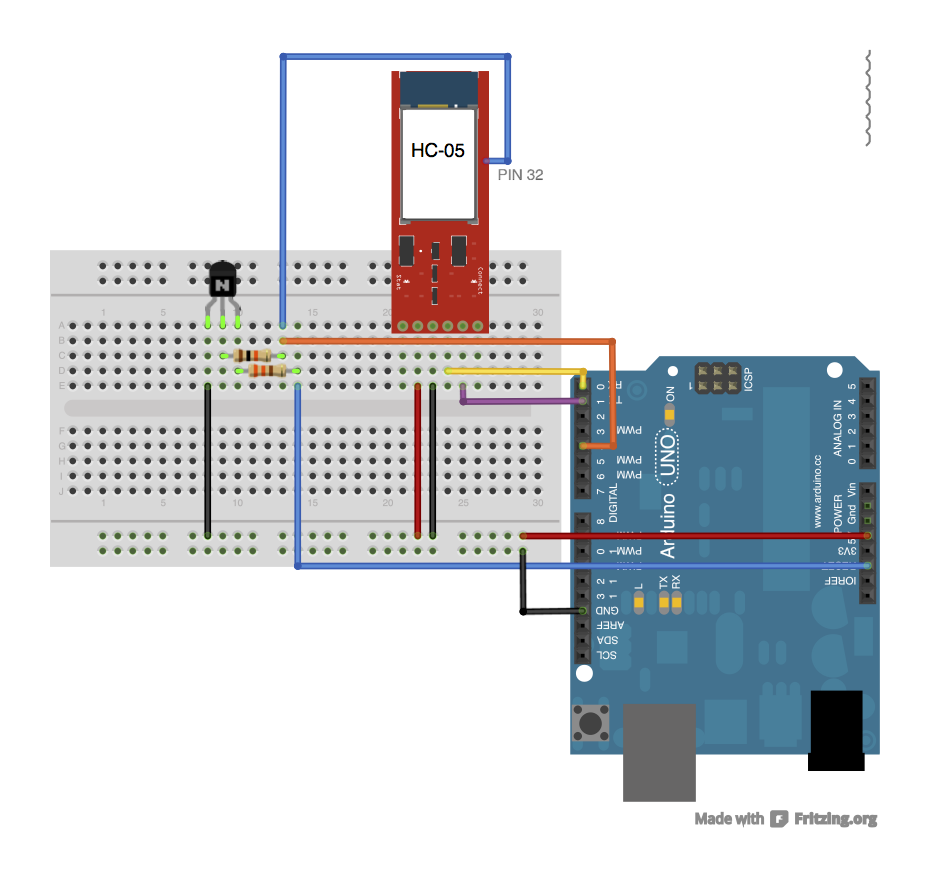
\includegraphics[scale=0.8]{images/wiring_hardReset.png}
        \captionof{figure}{How to wire the hard reset using the HC-05~~\cite{hc-05}.}
		\end{figure}
	
    \subsection{Security}
	Bluetooth itself provides security measures through channel encryption and pairing devices. In the case of
    critical devices, additional security might be needed. A simple way to incorporate this, would be to store a
    key in the EEP-ROM of the Arduino. The ComputerSerial library would then require authentication based on this
    key before allowing the initial soft reset. A QR code (this should not be plainly visible) could contain
    both the MAC address of the device and the required security details for ease of use, though a manual input
    method should also be available. This could easily be integrated with the regular connection management present
    in the application.\\
    
    However, this implementation is vulnerable to hard resets; if the device restarts on a Bluetooth connection, the
    security scheme is pointless. Because of this, the hard reset feature would have to be disabled on such devices,
    meaning the added security is at the expense of ease of use. This presents a second problem; without a way to be
    sure of automatic error recovery, even authenticated programming poses a risk to critical devices. Therefore, where more than paired device security is required, regular cabled programming is the safest way to go.
    
    \subsection{Protocols}
    The implementation targeted specifically the Optiboot boot loader used by many Arduinos. A subset of the STK500
    protocol is used for communicating with it. A factory pattern could be utilized to request a protocol capable of
    communicating with other boot loaders or full programmers (a separate chip doing the programming, requiring a
    full implementation of either v1 or v2 of STK500).
